\documentclass{article}

\usepackage{full page}

\usepackage{listings}
\usepackage{graphicx}
\usepackage{float}
\usepackage{caption}
\usepackage{subcaption}
\lstset{language=Java}

\title{Mazeworld Solution}
\author{Michelle Shu}

\begin{document}
\maketitle

\section{Introduction}

This report addresses several variations of a path-finding problem in which robots are to navigate a maze with obstacles from a start location to a goal location. I will use the A* search algorithm for this problem due to the efficiency and accuracy advantages it offers over uninformed search methods like breadth-first search and depth-first search, as described in the following section.

\section{A* Search}

A* search is one type of {\bf best-first search}, a general strategy of exploring graphs by choosing to expand the most promising nodes first. Variations of best-first search differ on the basis of the functions they use to decide which nodes are most promising. In the particular case of A*, nodes are chosen on the basis of the function $f(n) = d(n) + h(n)$, where $d(n)$ is the cost of reaching node $n$ from the starting position and $h(n)$ is a heuristic that estimates the distance from $n$ to the goal position. Thus, A* combines the best features of breadth-first search (which only uses the cost function, i.e. $f(n) = d(n)$) and greedy search (which uses only the heuristic, i.e. $f(n) = h(n)$). Including the cost of reaching the current node in the objective function increases the optimality of the path found, because it prevents the search from venturing too far from the start in a long winding path as sometimes may happen in greedy search. On the other hand, including the heuristic in the objective as well increases the efficiency of the search, as we are using additional information to point the search in the right direction.

My implementation of A* search is the function \verb`astarSearch` in \verb`InformedSearchProblem.java`. I used Java's PriorityQueue data structure to manage the nodes in the frontier and to choose which to expand next. The priority of a node is determined by the sum of the cost function from the start to the current node and a heuristic estimating the distance left to the goal.

\vspace{10mm}

\begin{lstlisting}
public List<SearchNode> astarSearch() {  
    resetStats();
    PriorityQueue<SearchNode> pq = new PriorityQueue<SearchNode>();
    HashMap<SearchNode, SearchNode> visited = 
        new HashMap<SearchNode, SearchNode>();
    
    pq.add(startNode);
    visited.put(startNode, startNode);
    
    while (! pq.isEmpty()) {
      incrementNodeCount();
      updateMemory(pq.size() + visited.size());
      
      SearchNode currentNode = pq.poll();
      SearchNode visitedNode = visited.get(currentNode);
      
      if (visitedNode != null && 
          visitedNode.getCost() < currentNode.getCost()) {
        continue; // ignore if already seen at lower cost.
      }
      
      if (currentNode.goalTest()) { // found goal, return the path
        return backchain(currentNode);
      }
      
      ArrayList<SearchNode> successors = currentNode.getSuccessors();
      for (SearchNode n : successors) {
        // Add the node if it has not been visited or if it was
        // previously found via a higher-cost path.
        SearchNode v = visited.get(n);
        if (v == null || v.getCost() > n.getCost()) {
          pq.add(n);
          visited.put(n, n);
          n.setParent(currentNode);
        }
      }
    }
    return null; // no path found
  }
\end{lstlisting}

\subsection{Updating cost of previously visited nodes}
As the search progresses, we may encounter a node that was previously visited, but via a lower-cost path than the original path on which it was found. In this case, we must revise it's that node's cost and and update its parent node to the new one corresponding to the lower cost. Unfortunately, it can be computationally expensive to locate the old node in our priority queue (internally represented as a heap), update its values and restructure the heap to maintain its ordering. 

An alternative method to achieve the same result is to simply not remove the old instance of the node, just inserting the new one and choosing to ignore the older one when it is polled from the priority queue. To this end, I chose to store all visited nodes in the HashSet called \verb`visited`. The cost of the node when it was found is recorded at the time it was initialized and before it was added to \verb`visited`. Thus, before adding a successor node to the frontier, we first check to see if it was already visited. If so, we compare its cost to the cost of the node that was visited. We only add the new node if it has a lower cost. Additionally, when removing a node from the frontier, we choose not to explore from it if it has a higher cost than an identical node in \verb`visited` (in this case, it is an old node we can choose to ignore).

\subsection{Results}

I applied A* search to the problem of a single robot navigating a maze from a start node to a goal node. Each node of this search problem represents a location (a $(x, y)$ coordinate pair of the robot. I used the Manhattan distance from the robot's location to the goal location as a heuristic. This heuristic is both admissible (shortest path possible regardless of obstacles, so always underestimates true distance to goal) and consistent (since it is directly related to physical distances, the triangle inequality holds).

The following results demonstrate the time and space complexities of the single robot A* search on a simple maze, in comparison to two uninformed search methods: DFS and BFS. As shown, BFS and A* both find shortest paths for this example. However, A* finds the goal significantly faster and does not need to use as much space, due to the information provided by the heuristic. DFS is fast, but finds a sub-optimal path since it is not rewarded for finding a short path.

\begin{figure}[!htb]
\centering
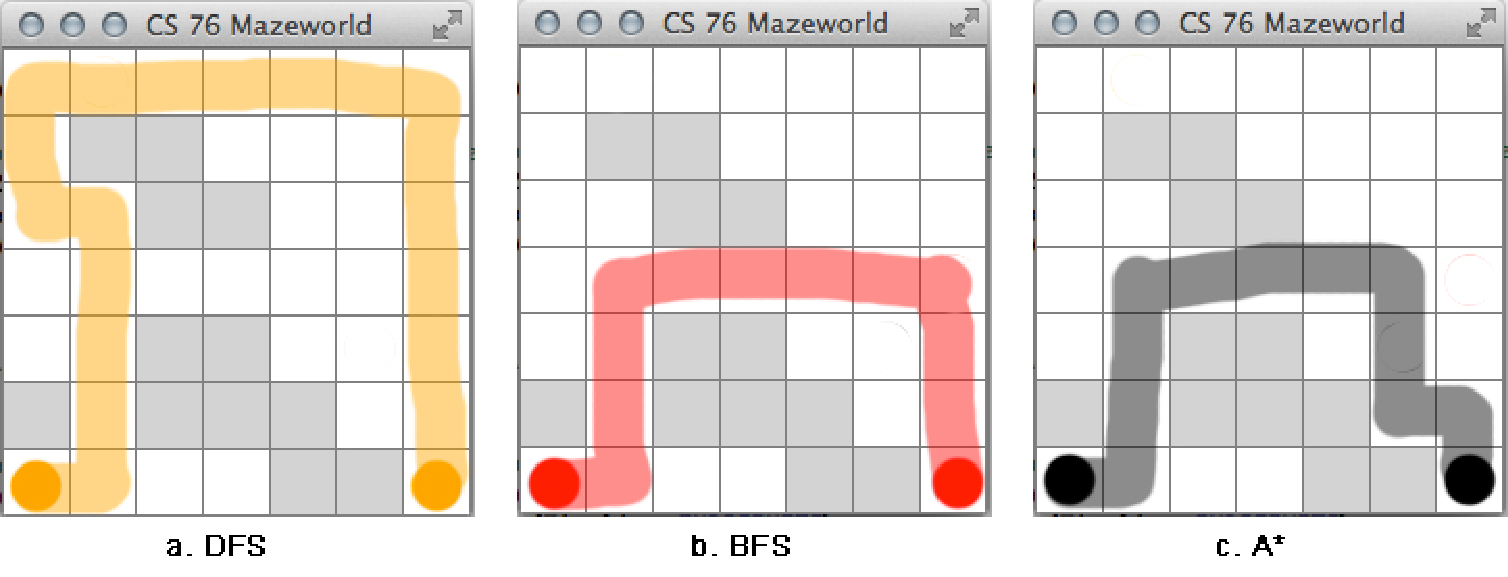
\includegraphics[scale=.55]{onerobot.pdf}
\caption{{\bf Comparison of search algorithms} Paths found by a. DFS, b. BFS and c. A* on a 7 x 7 maze.}
\end{figure}

\vspace{5mm}

{\setlength{\parindent}{0cm}
BFS:  \\
  Nodes explored during search: 37\\
  Maximum space usage during search: 41\\
DFS:  \\
  Nodes explored during search: 21\\
  Maximum space usage during search: 21\\
A*:  \\
  Nodes explored during search: 19\\
  Maximum space usage during search: 30\\
}
  
\section{Multi-robot coordination}
 
Now we extend the mazeworld problem to incorporate $k$ robots, instead of just one. We describe the locations of robot $i$ (where $i$ is an integer between $0$ and $k - 1$) with the coordinates $(x_i, y_i)$. We only allow the robots to move one at a time, taking turns sequentially. When its turn is up, a robot may choose to move any of 4 directions: North, South, East or West. Alternatively, it could choose not to move at all. Therefore, these are the only 5 possible transitions from one state to the next.

We incorporate each individual robot's location as well as an indicator of whose turn is up in the state representation. If there are $k$ robots overall, we will need $2k + 1$ dimensions to represent a state of the entire system ($2k$ for all $k$ robots' $(x, y)$ coordinates, plus an extra marker for the current robot to move). A rough upper bound on the number of possible states available is $O(n^{2k}*k)$. This is derived from reasoning that each robot can occupy any of $O(n^2)$ locations (any space on the board except spaces already occupied by obstacles and other robots), giving us the $O(n^{2k})$ term and it can be any of $k$ robots' turns, giving us the additional multiplier of $k$ for the result $O(n^{2k}*k)$.

A collision occurs whenever a robot's location is the same as the location of a wall (obstacle). This is an invalid state. If $n$ is much larger than $k$ and there are $w$ walls in the maze, we can expect about $O((k+w)^k*k)$ states to be collision states. This is because each robot can be colliding with up to $k - 1$ robots and $w$ walls, giving us the $O((k+w)^k)$ term for all $k$ robots, and this can happen on any of the $k$ robots' turns.

This analysis demonstrates that, for a maze with few walls, few robots and large $n$, the state space can be extremely large even after subtracting collision states. With $n = 100$ and $10$ robots, there are approximately $10^22$ possible states. It would clearly be infeasible to explore a graph of this size in its entirety with a undirected method like BFS (which puts you at risk of having to explore all the nodes in the state space).

Using A* can greatly reduce the computational costs of the multi-robot search, provided that we have a good heuristic function. In my implementation of A* for the multi-robot problem, I chose to use the sum of all robots' Manhattan distances as a heuristic. This is an appropriate choice, because as mentioned previously, Manhattan distances will always underestimate the true distance to the goal. Additionally, the sum of Manhattan distances is a monotonic (consistent) heuristic, meaning that it only decreases and never increases as we proceed along a path toward the goal. It is easy to see that this is true, because when any of the multiple robots moves closer to the goal, the sum of Manhattan distances only decreases.

My implementation of the multi-robot, save for the state representation, is similar to my solution to the single robot A* search. The major change is that the dimensions of the state representation have expanded to account for the additional robots' positions and to track which one is up to move. We reserve a dimension of the state representation for tracking the turn, so that we can easily compute the successors of a node and move the appropriate robot. This is done as follows in the function \verb`getSuccessors`:

\begin{lstlisting}
public ArrayList<SearchNode> getSuccessors() {
  ArrayList<SearchNode> successors = new ArrayList<SearchNode>();
  int r = state[2 * k]; // index of current robot
  
  for (int[] action: actions) {
    int xNew = state[r] + action[0];
    int yNew = state[k + r] + action[1];
    // make copy of current state to modify for successors
    int[] xStates = Arrays.copyOfRange(state, 0, k);
    int[] yStates = Arrays.copyOfRange(state, k, 2*k);
    
    if(maze.isLegal(xNew, yNew) && 
        ! this.robotsCollide(r, xNew, yNew)) { // collide with other robot?
      xStates[r] = xNew;
      yStates[r] = yNew;
      SearchNode succ = new MazeNode(xStates, yStates, (r + 1) % k,
          getCost() + 1.0);
      successors.add(succ);
    }  
  }
  
  // Also add current node to successors (choose no movement)
  int[] xStates = Arrays.copyOfRange(state, 0, k);
  int[] yStates = Arrays.copyOfRange(state, k, 2*k);
  successors.add(new MazeNode(xStates, yStates, (r + 1) % k, 
      getCost() + 1.0));
  return successors;
}
\end{lstlisting}

\subsection{Multi-Robot Search Results}

A* search was run on several example mazes of sizes ranging from 5x5 to 40x40 and a number of robots ($k$) ranging from 2 to 4. Mazes were designed with the following challenges in mind:

\begin{itemize}
  \item Can many robots navigate in small space?
  \item Can robots coordinate with one another when one needs to get out of the way so the other can pass?
  \item Can robots navigate efficiently (find optimal paths) through both side open spaces and narrow corridors?
\end{itemize}

Using the A* algorithm, I was able to generate satisfactory solutions to all the mazes created. Here are the figures of the robots' paths and the values describing the time and space efficiency of the searches.

\begin{figure}[!htb]
\centering
\begin{subfigure}{.5\textwidth}
  \centering
  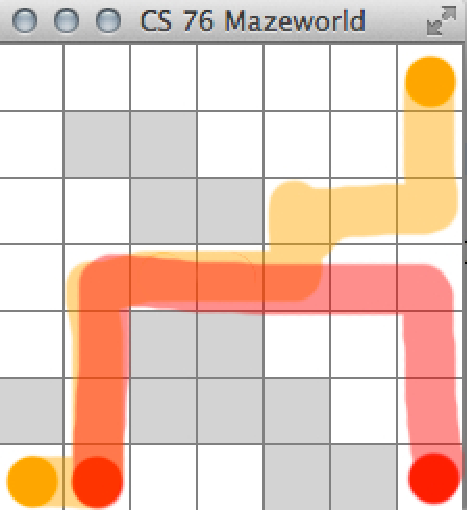
\includegraphics[scale=.65]{multimaze7.pdf}
  \caption{{\bf $k=2, n=7$} Nodes explored: 160; Max space: 454}
\end{subfigure}%
\begin{subfigure}{.5\textwidth}
  \centering
  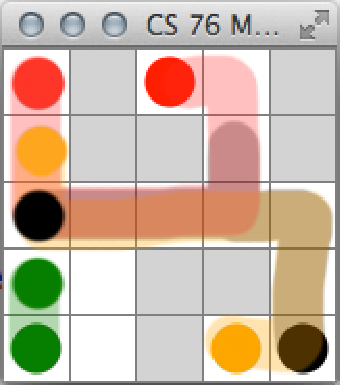
\includegraphics[scale=.65]{multimaze5.pdf}
  \caption{{\bf $k=4, n=5$} Nodes explored: 51936; Max space: 83282}
\end{subfigure}
\caption{Results of multi-robot A* search on small mazes}
\end{figure}

\begin{figure}[!htb]
\centering
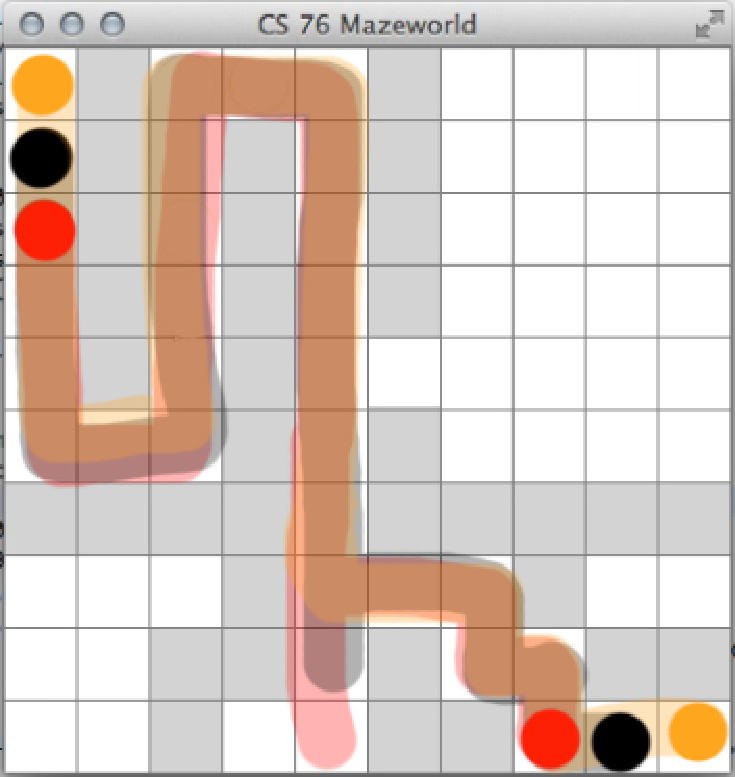
\includegraphics[scale=.65]{multimaze10.pdf}
\caption{{\bf $k=3, n=10$} Nodes explored: 8977; Max space: 12414}
\end{figure}

\begin{figure}[!htb]
\centering
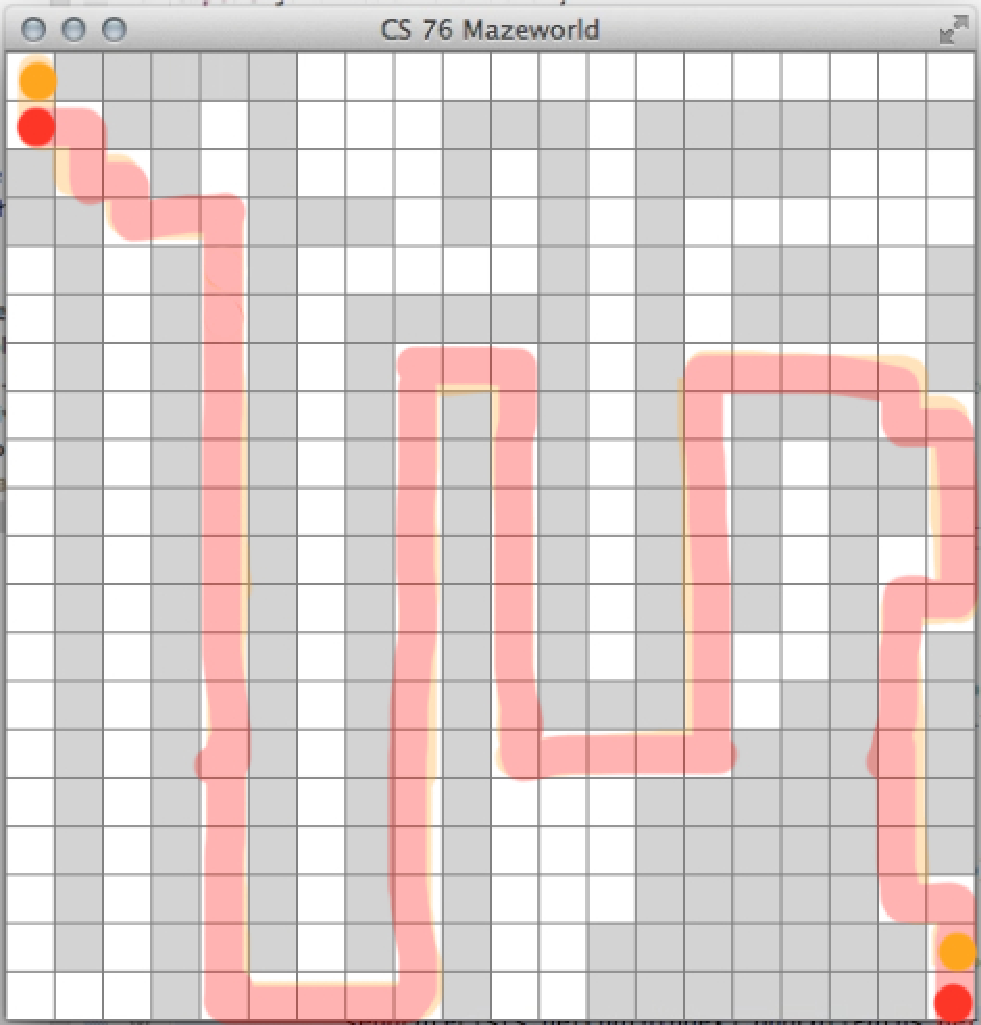
\includegraphics[scale=.7]{multimaze20.pdf}
\caption{{\bf $k=2, n=20$} Nodes explored: 63575; Max space: 66746}
\end{figure}

\begin{figure}[!htb]
\centering
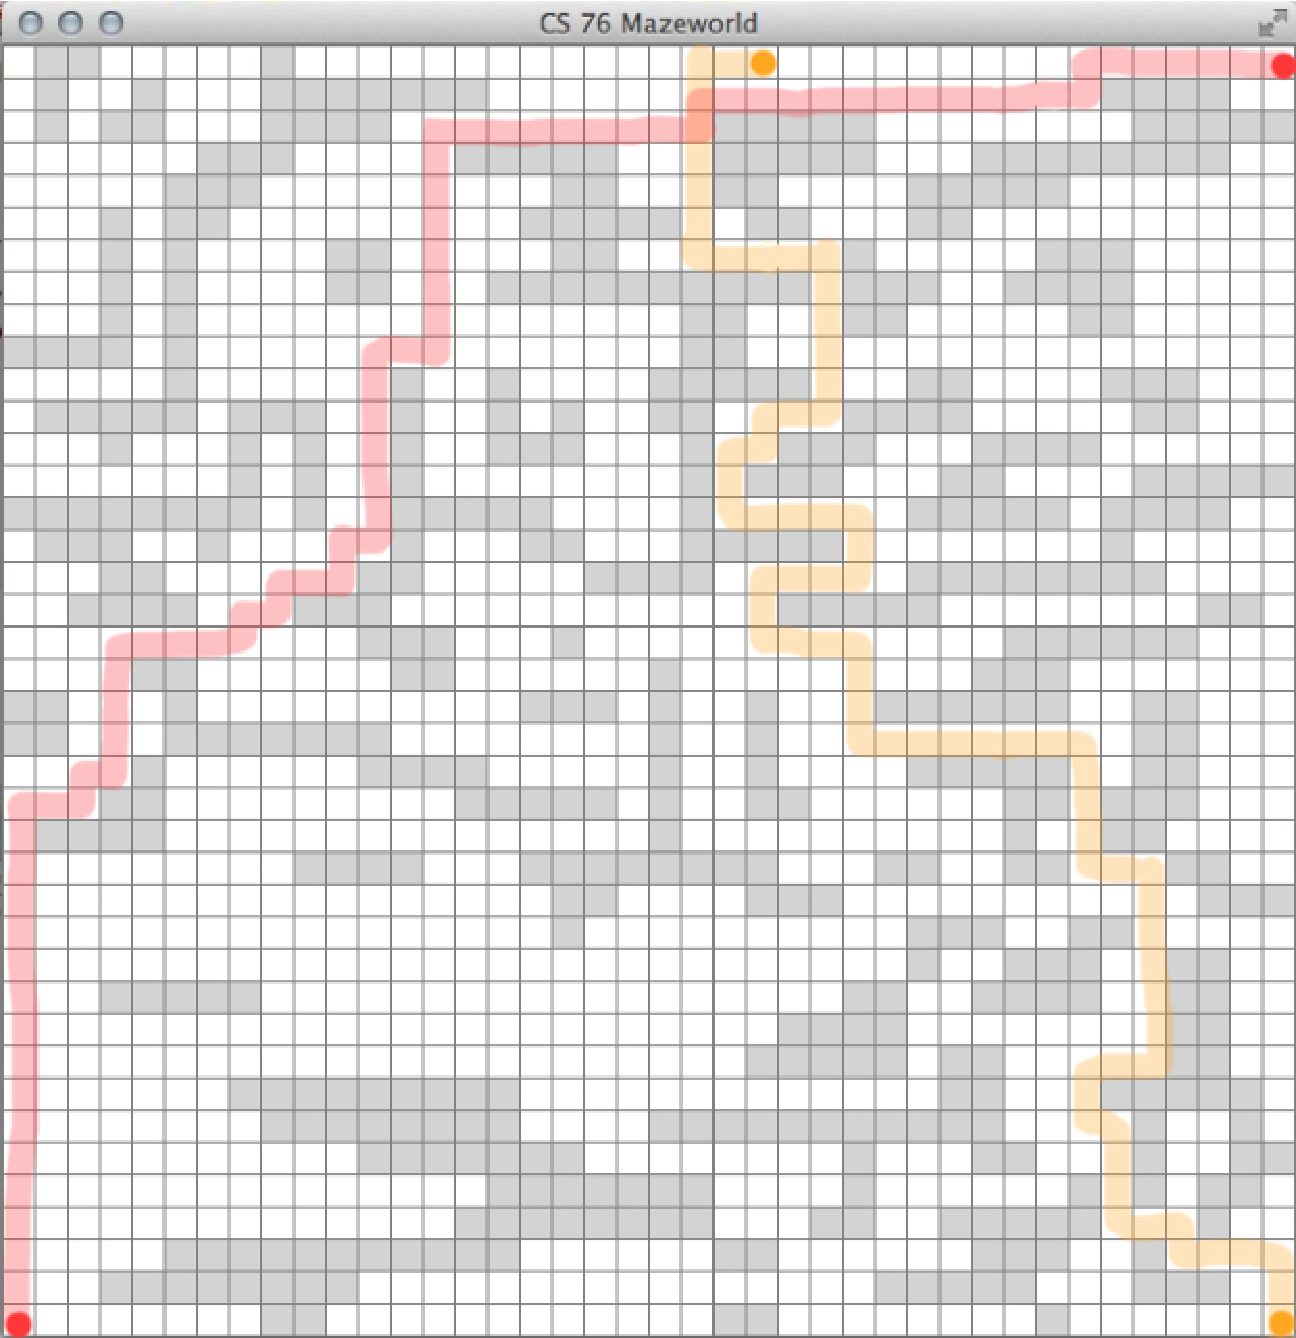
\includegraphics[scale=.75]{multimaze40.pdf}
\caption{{\bf $k=2, n=40$} Nodes explored: 98707; Max space: 124650}
\end{figure}

\subsection{Discussion of the 8-puzzle}

The 8-puzzle is a special case of this multi-robot search problem. It can be described as a 3x3 "maze" with no obstacles and 8 numbered robots placed within it. The size of the state space of the 8-puzzle is equivalent to the number of possible permutations of 9 distinct values or $9!=362880$ (treat the blank space as one of the values). The sum of Manhattan distances is also a valid heuristic for the 8-puzzle problem and it is indeed the heuristic that is commonly chosen for solving this problem via A* search. However, I suspect that the sum of Manhattan distances may grossly underestimate the true distance to the goal. Due to the major constraint of only having one free space on the board to move into, the pieces (robots) will almost surely each take paths that are much longer than the Manhattan distances to their goal locations. Practically, this may mean that the puzzle will take longer to solve using A* and this very optimistic heuristic.

We can empirically prove that the 8-puzzle state space consists of two disjoint sets of configurations that are reachable from one another. Theoretically, we could find the exact states belonging to one set by choosing a starting state at random and doing a breadth-first search from this state, recording all reachable states in a hash set. Then, we would generate random states until we find one that is not in the first set (not in the hash table from previous step) and do another breadth first search on this node, creating a separate hash set. If in the end, if the sizes of the two hash sets generated add up to $9!$ and neither one is empty, we could conclude that they together represent two disjoint sets that cover the entire state space.

\section{Blind robot with Pacman physics}

Suppose we now have a robot that is "blind" with no sensors. The robot can only sense the direction in which it is traveling and cannot respond to its environment. Therefore, the robot does not know when it has collided with an obstacle or wall. However, it does have an internal map of the maze.

In order for the blind robot to navigate to the goal location on the maze, it must first figure out where its own location is on the map. In the beginning, the robot has no information about where it is on the map, so its belief state (its perception of where it could possibly be) is a set of all valid locations on the map. The robot's first goal is to selects a sequence of actions (a plan) that, after completed, will narrow down its belief state to a single location. At this time, it will be absolutely certain of where it is, and from there on, it can use its knowledge of the map to navigate to the goal.

I use a different variation of A* search for the first part of this algorithm, generating a plan to narrow down the robot's current location. Each node in this search is a belief state: a set of nodes where the robot believes it may be. The successor of a node is given by the robot's deduction of its own location after moving in one of the four directions (north, south, east, west). In many cases, after moving, the robot can eliminate some location(s) from its belief state, becoming more certain of where it is. For example, if (0, 0) and (0, 1) are both valid locations on the maze and in the belief state, and the robot moves north, it can deduce that it cannot be in the (0, 0) location anymore, since it would have moved out of it.

We keep in mind a few simple rules that are key to this deductive process. For a direction of movement $<i, j>$ from location $(x, y)$:

\begin{itemize}
  \item If the robot can move in direction $<i, j>$ from $(x, y)$, we add $(x + i, y + j)$ to the belief state.
  \item If nothing moves into $(x, y)$ from $(x - i, y - j)$, then we eliminate $(x, y)$ from the belief state.
  \item If $(x - i, y - i)$ is also in the belief state, then we shift it by $<i, j>$ into the location previously occupied by $(x, y)$. We repeat for $(x - 2i, y - 2i)$, $(x - 3i, y - 3i)$, and so on as long as they are all in the belief state. So effectively, we just eliminate the last belief state location we come across in direction $<-i, -j>$.
\end{itemize}

I use the method \verb`getSuccessors` in \verb`BlindMazeProblem.java` to compute successors of belief states. \verb`getSuccessors` makes a copy of the current belief state and then for every direction of movement (action), it updates the belief state by considering the effect of the action on every location in the current belief state. The helper function \verb`updateHelperFunction` computes the proper update according to the rules listed above.

\begin{lstlisting}
public ArrayList<SearchNode> getSuccessors() {
  // For each possible action, check all locations in belief state to
  // see and add and eliminate new belief state locations accordingly
  ArrayList<SearchNode> succ = new ArrayList<SearchNode>();
  
  for (int[] action : actions) {
    int dx = action[0];
    int dy = action[1];
    
    HashSet<Location> stateCopy = new HashSet<Location>();
    for (Location l : this.state) {
      stateCopy.add(l);
    }
    updateBeliefState(stateCopy, dx, dy);
    BlindMazeNode newNode = new BlindMazeNode(stateCopy, this.minX,
        this.maxX, this.minY, this.maxY, this.cost + 1.0);
    
    // Update minX, maxX, minY, maxY for heuristic
    newNode.updateMinMax();
    newNode.setParent(this);
    succ.add(newNode);
  }
  return succ;
}


public void updateBeliefState(HashSet<Location> newState, int dx, int dy) {
  ArrayList<Location> toRemove = new ArrayList<Location>();
  ArrayList<Location> toAdd = new ArrayList<Location>();
  Iterator<Location> iter = state.iterator();
  
  while (iter.hasNext()) {
    Location l = iter.next();
    if (maze.isLegal(l.x + dx, l.y + dy)) {
      // Can now make this action into possibly new location
      toAdd.add(new Location(l.x + dx, l.y + dy));
      
      // If nothing moves into this location, remove it
      if (! maze.isLegal(l.x - dx, l.y - dy) || 
        ! state.contains(new Location(l.x - dx, l.y - dy))) {
        toRemove.add(l);
      }
      
      // If something can move into this location, shift
      // every preceding location over one.
      else if (state.contains(
          new Location(l.x - dx, l.y - dy))) {
        int i = l.x - 2 * dx;
        int j = l.y - 2 * dy;
        while (state.contains(new Location(i, j))) {
          i--;
          j--;
        }
        toRemove.add(new Location(i + 1, j + 1));
      }
    }
  }

  for (Location r : toRemove) {
    newState.remove(r);
  }
  for (Location a : toAdd) {
    newState.add(a);
  }
}
\end{lstlisting}

This A* search terminates when the robot has narrowed down its belief state to a size of 1. The only location left in its belief state at that point is the robot's true location. From here, the robot can navigate to the goal by using another A* search, the basic single robot A* search introduced in the first section of this report, because it now knows its start and goal locations.

\subsection{Blind robot heuristic}

For the A* search in which the robot deduces its own location, I used the heuristic $h(x) = (maxX - minX) + (maxY - minY) - 2$, where $minX$ and $maxX$ are the minimum and maximum x-coordinate of any location in the belief state and . This heuristic is a lower bound on the number of moves it takes from the current belief state to reduce the size of the belief state to 1. This is because each move can at most result in either the range of x-values or the range of y-values decreasing by 1. Thus, we need at the very least $maxX - minX - 1$ moves for the x range to be reduced to 1 and $maxY - minY - 1$ moves for the y range to be reduced to 1. Therefore, $h(x)$ is a lower bound for the distance to the goal and is therefore an admissible heuristic.

\subsection{Results}

Here is a visualization of the first phase of this search in which the blind robot reduces the size of its belief state by taking a sequence of actions.

\begin{figure}[!htb]
\centering
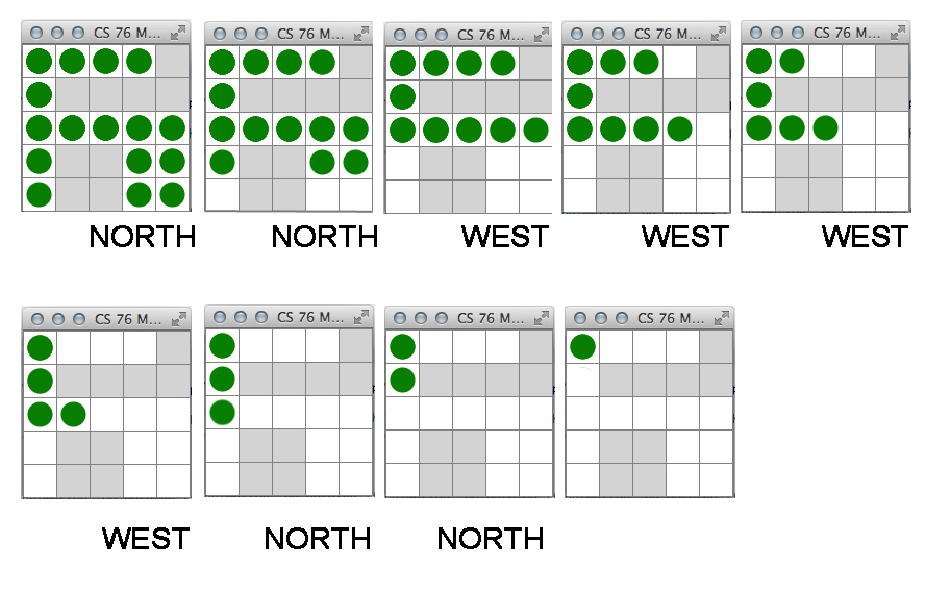
\includegraphics[scale=1]{blindrobot.pdf}
\caption{{\bf Blind robot belief state reduction.} Green dots represent locations where the robot believes it may be located at the present. The robot takes the actions displayed below each state to proceed to the following belief state.}
\end{figure}

{\setlength{\parindent}{0cm}
Nodes explored during search:  16\\
Maximum space usage during search 81\\
}

\subsection{Polynomial time blind robot planning}
A blind robot plan always exists if the maze is finite and the maze is contiguous. To see why this is true, we first observe that the locations in the belief state are all in the same connected component, so they can all reach each other. The size of the belief state can only decrease and never increase, so with enough time and actions, we will always converge on a belief state of size 1. (The decreases occur as two or more nodes that are next to each other "move" into a wall.)

Additionally, we can see that if we use the right algorithm, we can always find a plan for the robot to know its own location in polynomial time. This may be a surprise, because the number of possible belief states is exponential with respect to the size of the maze, but intuitively, we can think of it this way: if in the process of the search, the size of the belief state is decreasing frequently, the search space is continuously narrowed as we go. 

At any point during the search, we can guarantee that it is possible to reduce the size of the belief state if there are multiple locations in the belief state that are next to each other and at least one of these locations is adjacent to a wall of the maze. We can test if this is the case by trying up to four possible actions and seeing if any of them would shrink the belief state. (This takes time $O(n^2)$). If this isn't the case, we have individual locations in the belief state that are each adjacent to a wall, but separated, so we move them together by pushing them into a corner. Finding a path to do this takes also takes $O(n^2)$ time. So we have one of the two scenarios mentioned here for $O(n^2)$ nodes, giving us $O(n^4)$ runtime overall to find the location of the blind robot.


\section{References}

Introduction to A*. Amit Patel. http://theory.stanford.edu/\textasciitilde amitp/GameProgramming/AStarComparison.html\\
William Zhou's and Yu-Han Lyu's responses to my question on Piazza\\
Eva Xiao and I consulted each other.
\end{document}